% begin module derivatives-as-function-ex1
\begin{frame}
\begin{example}
The graph of a function $f$ appears below.  Use it to sketch the graph of the derivative $f'$.
\begin{columns}[c]
\column{.5\textwidth}
\psset{xunit=1cm, yunit=1cm}
\begin{pspicture}(-0.4,-1.5)(6.1,1.5)
\psframe*[linecolor=white](-0.4,-1.5)(6.1,1.5)
\tiny
\psaxes{<->}(0,0)(-0.1,-1.5)(6,1.5)
%Function formula: 1- ((x) ((x) (x)))-5 (x)+1/12 ((x) ((x) ((x) (x))))+23/6 ((x) (x)) 
\psplot[linecolor=red, plotpoints=1000]{0}{6}{x x mul 3.83333 mul x x mul x mul x mul 0.0833333 mul add x -5 mul add x x mul x mul -1 mul add 1 add } 
\uncover<4->{
\psline[linecolor=blue](0.5, -1.083333333)(1.5, -1.083333333)
\pscircle*[fillcolor=white, linecolor=blue](1, -1.083333333){0.07}
\rput[t](1, -1.2){\tiny $m=0$}
}

\uncover<6->{
\psline[linecolor=blue](2.5, 0.25)(3.5, 0.25)
\pscircle*[fillcolor=white, linecolor=blue](3, 0.25){0.07}
\rput[b](3, 0.4){\tiny $m=0$}
}

\uncover<8->{
\psline[linecolor=blue](4.5, -1.083333333)(5.5, -1.083333333)
\pscircle*[fillcolor=white, linecolor=blue](5, -1.083333333){0.07}
\rput[t](5, -1.2){\tiny $m=0$}
}
\uncover<11->{
\psline[linecolor=blue](1.646446609, -0.686886724)(2.353553391, 0.020220057) (2.353553391,-0.686886724)(1.646446609, -0.686886724)
\pscircle*[fillcolor=white, linecolor=blue](2, -0.333333333){0.07}
\rput[t](2, -0.8){\tiny $m=1$}
}
\uncover<14->{
\psline[linecolor=blue](4.353553391, -0.686886724)(3.646446609, 0.020220057) (3.646446609,-0.686886724)(4.353553391, -0.686886724)
\pscircle*[fillcolor=white, linecolor=blue](4, -0.333333333){0.07}
\rput[t](4, -0.8){\tiny $m=1$}
}
\end{pspicture}
%\ \only<handout:0| -3>{%
%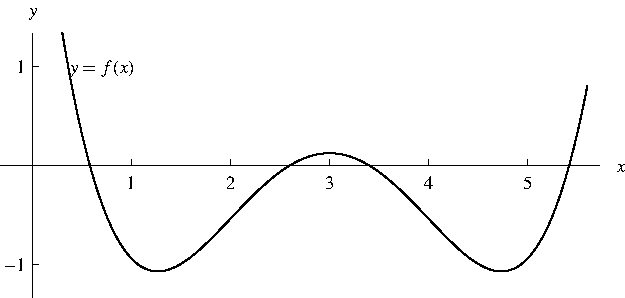
\includegraphics[height=2.9cm]{derivatives/pictures/03-02-ex1fa.pdf}%
%}%
%\only<handout:0| 4-5>{%
%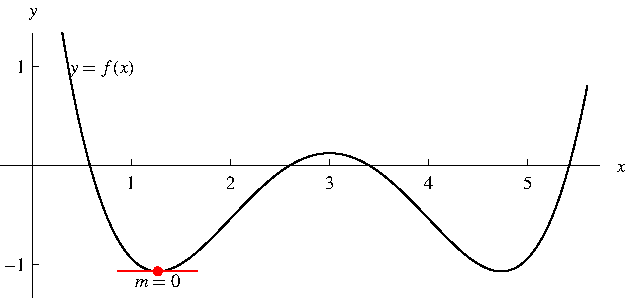
\includegraphics[height=2.9cm]{derivatives/pictures/03-02-ex1fb.pdf}%
%}%
%\only<handout:0| 6-7>{%
%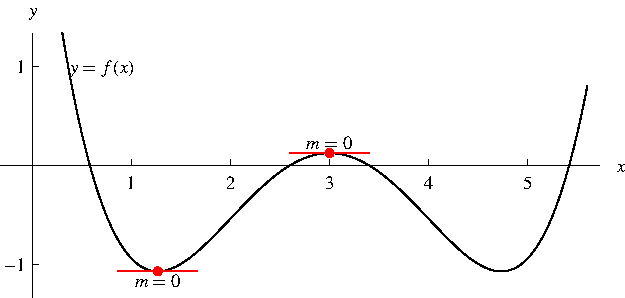
\includegraphics[height=2.9cm]{derivatives/pictures/03-02-ex1fc.pdf}%
%}%
%\only<handout:0| 8-10>{%
%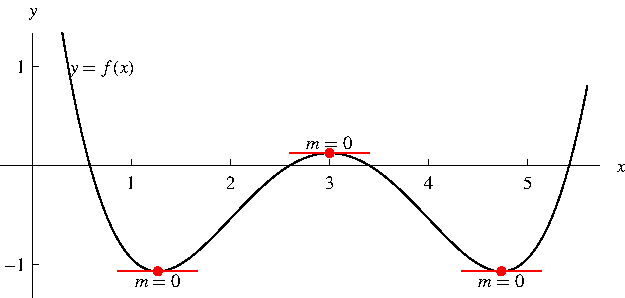
\includegraphics[height=2.9cm]{derivatives/pictures/03-02-ex1fd.pdf}%
%}%
%\only<handout:0| 11-13>{%
%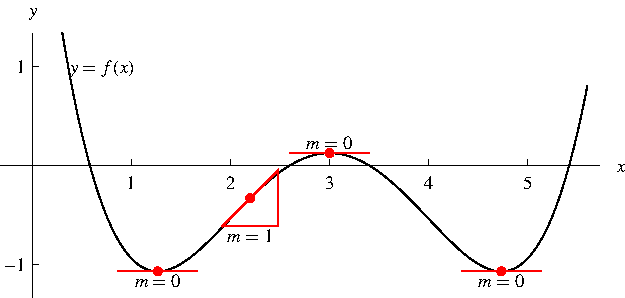
\includegraphics[height=2.9cm]{derivatives/pictures/03-02-ex1fe.pdf}%
%}%
%\only<14->{%
%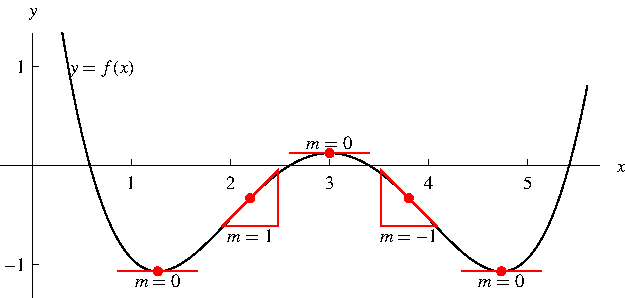
\includegraphics[height=2.9cm]{derivatives/pictures/03-02-ex1ff.pdf}%
%}%
%\ \only<handout:0| -4>{%
%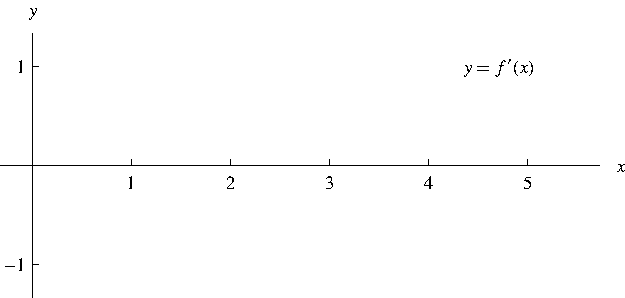
\includegraphics[height=2.9cm]{derivatives/pictures/03-02-ex1fprimea.pdf}%
%}%
%\only<handout:0| 5-6>{%
%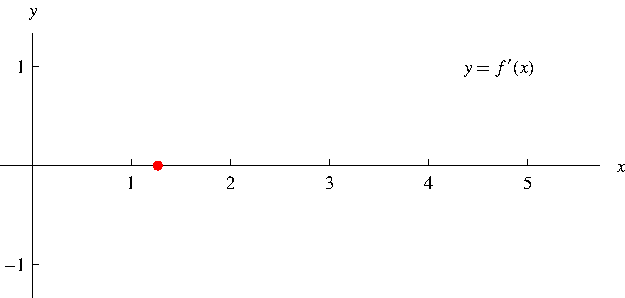
\includegraphics[height=2.9cm]{derivatives/pictures/03-02-ex1fprimeb.pdf}%
%}%
%\only<handout:0| 7-8>{%
%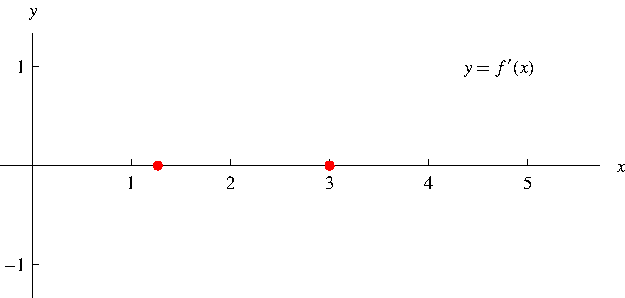
\includegraphics[height=2.9cm]{derivatives/pictures/03-02-ex1fprimec.pdf}%
%}%
%\only<handout:0| 9-11>{%
%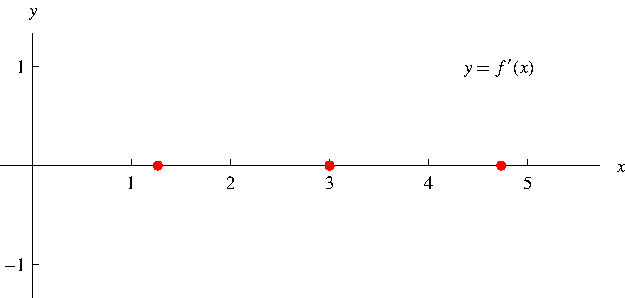
\includegraphics[height=2.9cm]{derivatives/pictures/03-02-ex1fprimed.pdf}%
%}%
%\only<handout:0| 12-14>{%
%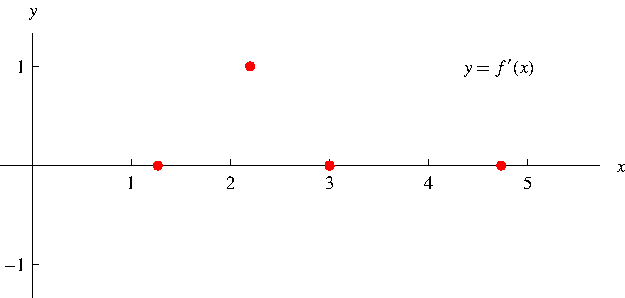
\includegraphics[height=2.9cm]{derivatives/pictures/03-02-ex1fprimee.pdf}%
%}%
%\only<handout:0| 15-17>{%
%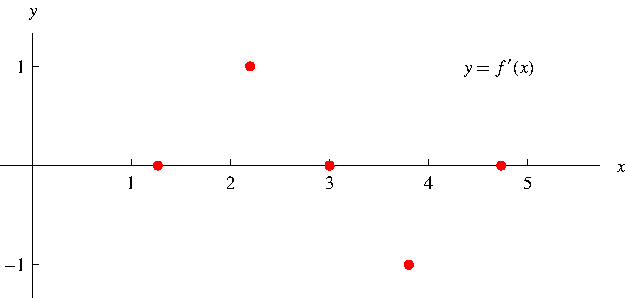
\includegraphics[height=2.9cm]{derivatives/pictures/03-02-ex1fprimef.pdf}%
%}%
%\only<18->{%
%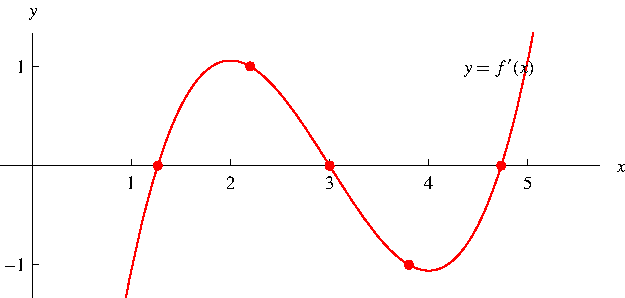
\includegraphics[height=2.9cm]{derivatives/pictures/03-02-ex1fprimeg.pdf}%
%}%



\psset{xunit=1cm, yunit=1cm}
\begin{pspicture}(-0.4,-2)(6.1,2)
\psframe*[linecolor=white](-0.4,-2)(6.1,2)
\tiny
\psaxes{<->}(0,0)(-0.1,-2)(6,2)
%Function formula: -5-3 ((x) (x))+23/3 (x)+1/3 ((x) ((x) (x))) 
\uncover<18->{
\psplot[linecolor=blue, plotpoints=1000]{0.5}{5.5}{x x mul x mul 0.333333 mul x 7.66667 mul add x x mul -3 mul add -5 add }
}
\uncover<5->{
\pscircle*[fillcolor=white, linecolor=blue](1, 0){0.07}
}
\uncover<7->{
\pscircle*[fillcolor=white, linecolor=blue](3, 0){0.07}
}
\uncover<9->{
\pscircle*[fillcolor=white, linecolor=blue](5, 0){0.07}
}
\uncover<12->{
\pscircle*[fillcolor=white, linecolor=blue](2, 1){0.07}
}
\uncover<15->{
\pscircle*[fillcolor=white, linecolor=blue](4, -1){0.07}
}
\end{pspicture}  
\column{.5\textwidth}
\begin{itemize}
\item<2->  Find the points where the tangent is horizontal ($m = 0$).
\item<3->  That is where $f'$ is $0$.
\item<10->  Where the slope of the tangent to $f$ is $1$, $f'$ is $1$.
\item<13->  Where the slope of the tangent to $f$ is $-1$, $f'$ is $-1$.
\item<16->  Where the slope of the curve is negative, $f'$ is negative.
\item<17-18>  Where the slope of the curve is positive, $f'$ is positive.
\end{itemize}
\end{columns}
\end{example}
\end{frame}
% end module derivatives-as-function-ex1
